% Created 2023-07-30 Sun 17:36
% Intended LaTeX compiler: pdflatex
\documentclass[11pt]{article}
\usepackage[utf8]{inputenc}
\usepackage[T1]{fontenc}
\usepackage{graphicx}
\usepackage{longtable}
\usepackage{wrapfig}
\usepackage{rotating}
\usepackage[normalem]{ulem}
\usepackage{amsmath}
\usepackage{amssymb}
\usepackage{capt-of}
\usepackage{hyperref}
\usepackage{minted}
\usepackage[a4paper]{geometry}
\usepackage{mathtools}
\author{Alexander Huss}
\date{\today}
\title{Parton Distribution Functions}
\hypersetup{
 pdfauthor={Alexander Huss},
 pdftitle={Parton Distribution Functions},
 pdfkeywords={},
 pdfsubject={},
 pdfcreator={Emacs 28.2 (Org mode 9.7)}, 
 pdflang={English}}
\begin{document}

\maketitle
\tableofcontents



\section{Introduction}
\label{sec:org76b74a7}
We will call the \href{https://lhapdf.hepforge.org/}{LHAPDF} library from python to evaluate parton distribution functions and play around with them a bit.

\section{Evaluating PDFs}
\label{sec:orge6e5fa1}
Let's have a look at one specific PDF set \texttt{PDF4LHC21\_40}

\begin{minted}[frame=lines,fontsize=\scriptsize]{python}
import lhapdf
import numpy as np

lhapdf.setVerbosity(0)
pdf = lhapdf.mkPDF("PDF4LHC21_40", 0)
if qlog:
    xs = [x for x in np.logspace(-5, 0, 50)]
else:
    xs = [x for x in np.linspace(0, 1, 50)]
res = np.empty([len(xs),6])
for ix, x in enumerate(xs):
    fac = 1. #1./x
    res[ix,0] = x
    res[ix,1] = q
    res[ix,2] = fac*(pdf.xfxQ(2, x, q) - pdf.xfxQ(-2, x, q))  # valence up-quark
    res[ix,3] = fac*(pdf.xfxQ(1, x, q) - pdf.xfxQ(-1, x, q))  # valence down-quark
    res[ix,4] = fac*(pdf.xfxQ(0, x, q))  # gluon (or `21`)
    res[ix,5] = fac*(
         2.*pdf.xfxQ(-2, x, q)
        +2.*pdf.xfxQ(-1, x, q)
        +pdf.xfxQ(3, x, q)+pdf.xfxQ(-3, x, q)
        +pdf.xfxQ(4, x, q)+pdf.xfxQ(-4, x, q)
        +pdf.xfxQ(5, x, q)+pdf.xfxQ(-5, x, q)
    )  # sum over all see quarks
return res
\end{minted}

\begin{center}
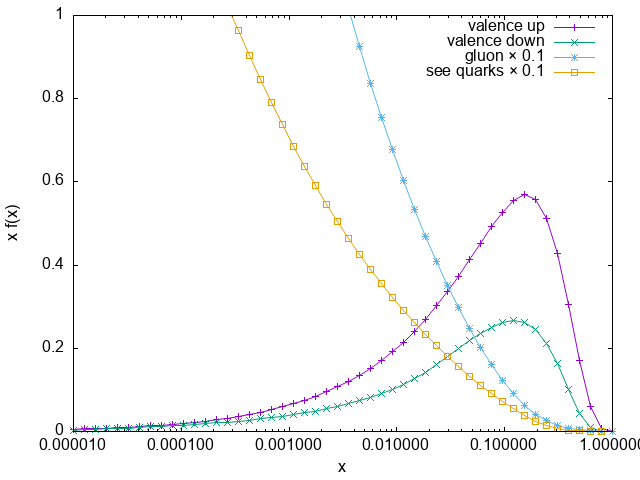
\includegraphics[width=.9\linewidth]{pdf_xfx.png}
\end{center}

\begin{quote}
\begin{itemize}
\item Change the scale in the figure from 10 to 100 GeV or even to 1 TeV; adjust the scaling factor as necessary.
How does the distributions change?
Does it correspond to the expectation of the QCD improved parton model?
\end{itemize}
\end{quote}

\section{The quantum numbers of the proton}
\label{sec:org910f48a}
The quantum numbers of the proton are determined by the valence quarks, p=(uud).
Given that PDFs are \emph{number densities} for the constituent partons, the following flavour sum rules hold:
\begin{align}
  \int_0^1\mathrm{d}x \Bigl(
    f_{\mathrm{u}\vert\mathrm{p}}(x)
  - f_{\bar{\mathrm{u}}\vert\mathrm{p}}(x)
  \Bigr)
  &= 2, &
  \int_0^1\mathrm{d}x \Bigl(
    f_{\mathrm{d}\vert\mathrm{p}}(x)
  - f_{\bar{\mathrm{d}}\vert\mathrm{p}}(x)
  \Bigr)
  &= 1,
  \\
  \int_0^1\mathrm{d}x \Bigl(
    f_{\mathrm{q}\vert\mathrm{p}}(x)
  - f_{\bar{\mathrm{q}}\vert\mathrm{p}}(x)
  \Bigr)
  &= 0 \quad \forall q \notin \{\mathrm{u},\,\mathrm{d}\}
\end{align}
Let's see if these hold for one of the global PDF sets:
\begin{minted}[frame=lines,fontsize=\scriptsize]{python}
import lhapdf
import math
import scipy
lhapdf.setVerbosity(0)
pdf = lhapdf.mkPDF("PDF4LHC21_40", 0)
res = list()
for id,label in [(1,"d"),(2,"u"),(3,"s"),(4,"c"),(5,"b")]:
    int_res = scipy.integrate.quad(lambda x : (pdf.xfxQ(id, x, q)-pdf.xfxQ(-id, x, q))/x, 1e-6, 1, limit=100, epsrel=1e-3)
    #print(int_res)
    res.append( (label, int_res[0]) )
return res
\end{minted}

\begin{center}
\begin{tabular}{lr}
d & 0.9867274422876251\\[0pt]
u & 1.9924213767549757\\[0pt]
s & 0.0037080323432484596\\[0pt]
c & -0.00018756880668407142\\[0pt]
b & -8.819432616743546e-05\\[0pt]
\end{tabular}
\end{center}

\section{Momentum sum rules}
\label{sec:orgbeb4503}
The parton \(a\) carries a momentum fraction \(x_a\) of the parent hadron, \(p_a^\mu=x_a\,P^\mu\).
Therefore, the momentum density associated with that parton is given by \$x\textsubscript{a$\backslash$,f}\textsubscript{a\(\vert{}\) H}(x\textsubscript{a}).
Since the sum over all parton momenta must sum back up to the parent hadron one, the PDF sets satisfy a \emph{momentum sum rule} (in \(\overline{\text{MS}}\)):
\begin{align}
  \sum_a \int_0^1 \mathrm{d}x_a \; x_a\,f_{a\vert H}(x_a)
  &= 1
\end{align}

Let's see how the momenta are distributed across different flavours
\begin{minted}[frame=lines,fontsize=\scriptsize]{python}
import lhapdf
import math
import scipy
lhapdf.setVerbosity(0)
pdf = lhapdf.mkPDF("PDF4LHC21_40", 0)
res = list()
int_sum = [0.,0.]
for id,label in [(-5,"bb"),(-4,"cb"),(-3,"sb"),(-2,"ub"),(-1,"db"),(0,"g"),(1,"d"),(2,"u"),(3,"s"),(4,"c"),(5,"b")]:
    int_res = scipy.integrate.quad(lambda x : pdf.xfxQ(id, x, q), 1e-6, 1, limit=100, epsrel=1e-3)
    int_sum[0] += int_res[0]
    int_sum[1] += int_res[1]**2
    #print(int_res)
    res.append( (label, "{:.0f}%".format(int_res[0]*100.)) )
res.append( ("SUM", "{:.0f}%".format(int_sum[0]*100.)) )
return res
\end{minted}

\begin{center}
\begin{tabular}{ll}
bb & 1\%\\[0pt]
cb & 2\%\\[0pt]
sb & 3\%\\[0pt]
ub & 4\%\\[0pt]
db & 4\%\\[0pt]
g & 47\%\\[0pt]
d & 11\%\\[0pt]
u & 22\%\\[0pt]
s & 3\%\\[0pt]
c & 2\%\\[0pt]
b & 1\%\\[0pt]
SUM & 100\%\\[0pt]
\end{tabular}
\end{center}

So the gluon actually carries almost \(50\%\) of the proton's momentum!
The up quark, with \(\sim20\%\), has the second largest contribution, followed by the down-quark \$\(\sim\)\$half the size of the up (which makes sense as p=(uud)).

\begin{quote}
\begin{itemize}
\item Vary the scale and see how the momentum composition of the proton changes.
How robust are the numbers?
\end{itemize}
\end{quote}
\end{document}